\documentclass[12pt,a4paper]{article}
\usepackage[utf8]{inputenc}
\usepackage[T1]{fontenc}
\usepackage[spanish]{babel}
\usepackage{booktabs}

\usepackage{amsmath}
\usepackage{amssymb}

\usepackage{graphicx}
\usepackage{float}

\usepackage{geometry}
\geometry{
left=2.5cm,
right=2.5cm,
top=2.5cm,
bottom=2.5cm
}

\begin{document}

\begin{titlepage}
\centering
\vspace*{1.5cm}

{\Large\textbf{Proyecto 01}\par}

\vspace{0.5cm}
\rule{10cm}{0.3pt}

\vspace{1.5cm}

{\LARGE\textbf{Fractales}\par}

\vspace{0.5cm}
\rule{10cm}{0.3pt}

\vspace{2cm}

{\Large Temas selectos de matematicas: Probabilidad \par}

\vspace{0.3cm}
{\large Maestría en Procesamiento de Señales\par}
{\large UNAM, 2027-1\par}

%\vfill

\vspace{4cm}

{\Large\textbf{Equipo:}\par}
\vspace{0.5cm}
Hernandez AbarcaAngel Miguel \\
\vspace{0.3cm}
Martinez Ramirez Jorge Fidel \\
\vspace{0.3cm}
Velasco Pedroza Gimena Alejandra

\vspace{2cm}

\end{titlepage}


\newpage
\section*{1. Introduccion}

Los fractales son estructuras geometricas que presentan patrones capaces de repetirse a diferentes escales. A pesar de que pueden presentar una geometria visual compleja, muchas de estas estructuras pueden generarse mediante reglas matematicas relativamente sencillas. \\

Una de las herramientas utilizadas para la generacion de fractales son los Sistemas de funciones iteradas (IFS), estos metodos se basan en la iteracion de una serie de transformaciones afines que, al aplicarse repetidamente, producen patrones denominados fractales, ademas encuentra aplicaciones en campos tan diversos como el procesamiento de imagenes, la modelacion de estructuras naturales y la generacion de grafos en computacion grafica. \\

En este trabajo, se explora la implementacion de los metodos mencionados anteriormente (IFS) para la creacion de fractales y estudiar el efecto que tienen tantos las probabilidades de seleccion de las transformaciones como el numero de iteraciones sobre la estructura resultante.

\section*{2. Objetivo}

\subsection*{2.1 Objetivo General}

Aplicar Sistemas de Funciones Iteradas (IFS) para la generación de fractales. Conocer Matlab para la
generación de variables aleatorias (v.a.) de distribución uniforme. Aplicar instrucciones histogram, rand,
unifrnd, y scatter.

\subsection*{2.2 Objetivos Particulares}

\begin{itemize}
    \item Comprender el fundamento matematico de los Sistemas de Funciones Iteradas (IFS).
    \item Utilizar variables aleatorias con distribucion uniforme para seleccionar las transformaciones.
    \item Generar y comparar diferentes estructuras fractales mediante procesos iterativos utilizando diferentes cantidades de puntos (10,000 . 100,000 . 1,000,000).
    \item Analizar el tiempo de procesamiento requerido para generar las diferentes estructuras.
\end{itemize}

\section*{3. Esquema IFS (Iterated Functions Systems)}

En general, un Sistema de Funciones Iteradas esta constituido por un conjunto de transformaciones, ya sea a una imagen (matriz) o como es el caso de este trabajo, a un punto. Las transformaciones son de $\mathbb{R}^2 \rightarrow \mathbb{R}^2$ y tienen la forma:

\begin{equation}
    w
\begin{pmatrix}
    x\\
    y
\end{pmatrix}
=
\begin{pmatrix}
    a & b\\
    c & d
\end{pmatrix}
\begin{pmatrix}
    x\\
    y
\end{pmatrix}
+
\begin{pmatrix}
    e\\
    f
\end{pmatrix}
\end{equation}


donde $a,b,c,d,e,f,g \in \mathbb{R}.$ \\

Por lo tanto, un sistema IFS puede tener $w_n$ transformaciones y el efecto que forman las n transformaciones se puede expresar como la unión de todas las transformaciones, expresado matemáticamente
como. 
\begin{equation}
    W(.)= \bigcup_{i} w_n
\end{equation}


En cada iteracion se selecciona una de las transformaciones y se aplica al punto actual:

\begin{equation}
    P_{n+1}=T_i(P_n).
\end{equation}

La particularidad de la metodologia utilizada en esta practica es que la seleccion de $T_i$ se realiza mediante una variable aleatoria.\\

Para estos sistemas, es importante notar que al iterar los sistemas hasta un número considerablemente alto, notamos como se formaran patrones repetitivos, es decir, fractales, por lo que estos sistemas pueden
ser utilizados para generar fractales.

\section*{4. Metodologia}

El procesamiento general utilizado para la generacion de los fractales fue el siguiente.

\subsection*{4.1 Inicializacion}

Primero se establecio un punto inicial en el plano, el primer algoritmo consta de tomar un punto arbitario y aplicarle un sistema IFS donde la transformacion a elegir se escogeria mediante la probabilidad $p_i > 0$ tal que $\sum_{i} = 1^N p_i = 1$. \\

Este punto representa el estado inicial del proceso iterativo.
 
\subsection*{4.2 Generacion de la variable aleatoria}

En cada iteracion se genero una variable aleatoria con distribucion uniforme en el intervalo $[0,1]$.

El valor obtenido permitio determinar cual de las transformaciones disponibles debia aplicarse.

\subsection*{4.3 Seleccion de la transformacion}

El valor de $U$ se comparo con los intervalos establecidos para cada transformacion.

La transformacion seleccionada depende, por lo tanto, de la probabilidad asignada a cada funcion.
\newpage
\subsection*{4.4 Transformacion del punto}

Una vez seleccionada la transformacion, se aplico al punto actual:

\begin{equation}
    P_{n+1}=T_i(P_n).
\end{equation}

El resultado constituye el nuevo punto de la secuencia.

\subsection*{4.5 Repeticion}

El punto obtenido se utilizo como entrada para la siguiente iteracion.
El procedimiento se repitio hasta obtener la cantidad de puntos deseada.
Para esta practica se realizaron simulaciones con la siguiente cantidad de puntos:
\begin{itemize}
    \item $10\,000$ puntos,
    \item $100\,000$ puntos,
    \item $1\,000\,000$ puntos,
\end{itemize}

El incremento en el numero de puntos permitio observar como la estructura fractal adquiere una mayor densidad y definicion conforme la cantidad de puntos aumento.

\section*{5. Aplicacion de fractales}

\subsection*{5.1 Generacion de paisajes y estructuras 3D}

Una de las aplicaciones de los fractales se encuentra en la computación gráfica, ya que se utilizan modelados fractales para la generación de texturas irregulares, como los paisajes, árboles, etc.

\subsection*{5.2 Modelado de fenomenos o figuras naturales}

En la naturaleza se encuentran figuras irregulares que pueden ser descritas mediante modelos fractales, ya sean contornos como la superficie de un terreno como una isla, hasta el modelado de la arteria carótida de un ser humano, posibilitando la evaluación de la eficacia de las intervenciones quirúrgicas con una buena aproximación matemática

\section*{6. Empleo de las instrucciones de Matlab(Octave)}

Para poder realizar este trabajo, se hizo uso de las siguientes funciones de matlab.

\begin{itemize}
    \item $histogram(x):$ crea una grafica de histograma de $x$.
    \item $rand(a,b):$ devuelve una matriz de $a * b$ con números aleatorios entre 0 y 1 con una distribucion uniforme.
    \item $plot(,x,y):$ crea una grafica de lineas en 2D de los datos $Y$ frente a $X$.
    \item $scater(x,y):$ crea un diagrama de dispersion con marcadores circulares en las ubicaciones especificadas por los vectores $x$ e $y$.
\end{itemize}

\section*{7. Resultados}
\subsection*{7.1 Helecho de Barnsley}

El primer fractal generado fue el Helecho de Barnsley. Para su construccion
se utilizaron cuatro transformaciones afines. Cada transformacion cuenta con una probabilidad diferente de seleccion. La variable aleatoria $U$ determina cual de las cuatro transformaciones se aplica en cada iteracion. Los intervalos de selección establecidos fueron:

\begin{equation}
U<0.01,
\end{equation}

\begin{equation}
0.01\leq U<0.86,
\end{equation}

\begin{equation}
0.86\leq U<0.93,
\end{equation}

\begin{equation}
U\geq0.93.
\end{equation}

Esto significa que la segunda transformación presenta una frecuencia de seleccion considerablemente mayor que las demas. La combinación de las cuatro transformaciones produce la estructura característica del helecho.

\subsubsection*{7.1.1 Resultados}

\begin{figure}[H]
    \centering
    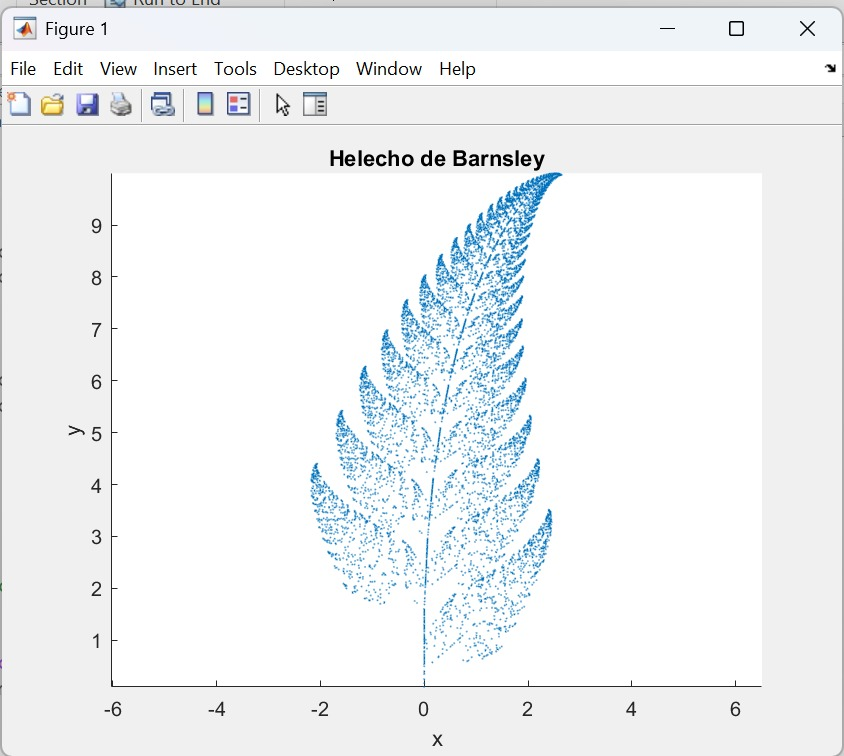
\includegraphics[width=0.75\textwidth]{helecho_10_000.jpeg}
    \caption{Helecho de Barnsley generado con 10\,000 puntos.}
    \label{fig:barnsley10000}
\end{figure}

\begin{figure}[H]
    \centering
    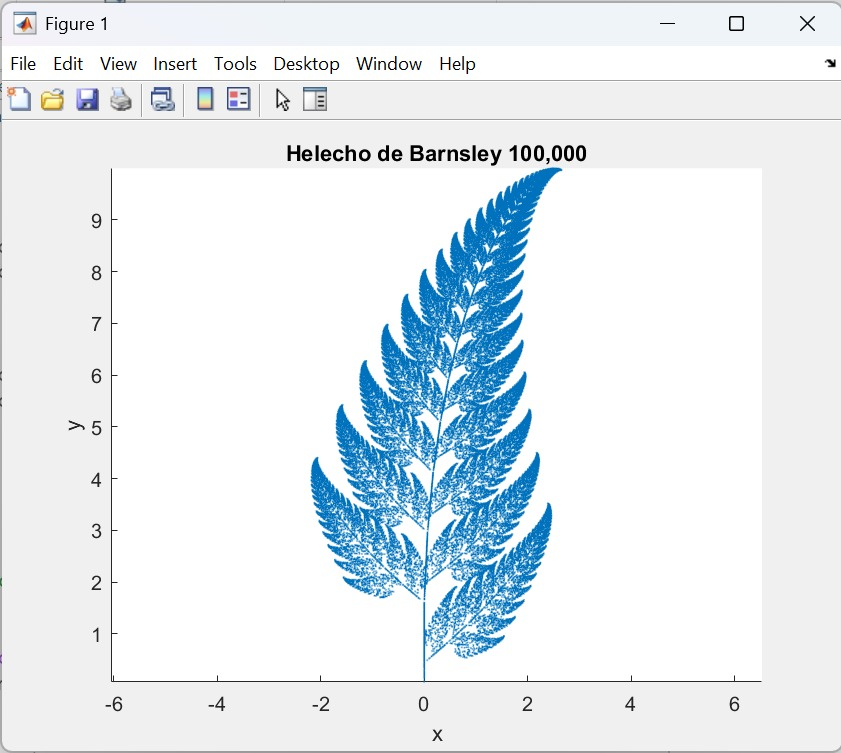
\includegraphics[width=0.75\textwidth]{helecho_100_000.jpeg}
    \caption{Helecho de Barnsley generado con 100\,000 puntos.}
    \label{fig:barnsley100000}
\end{figure}

\begin{figure}[H]
    \centering
    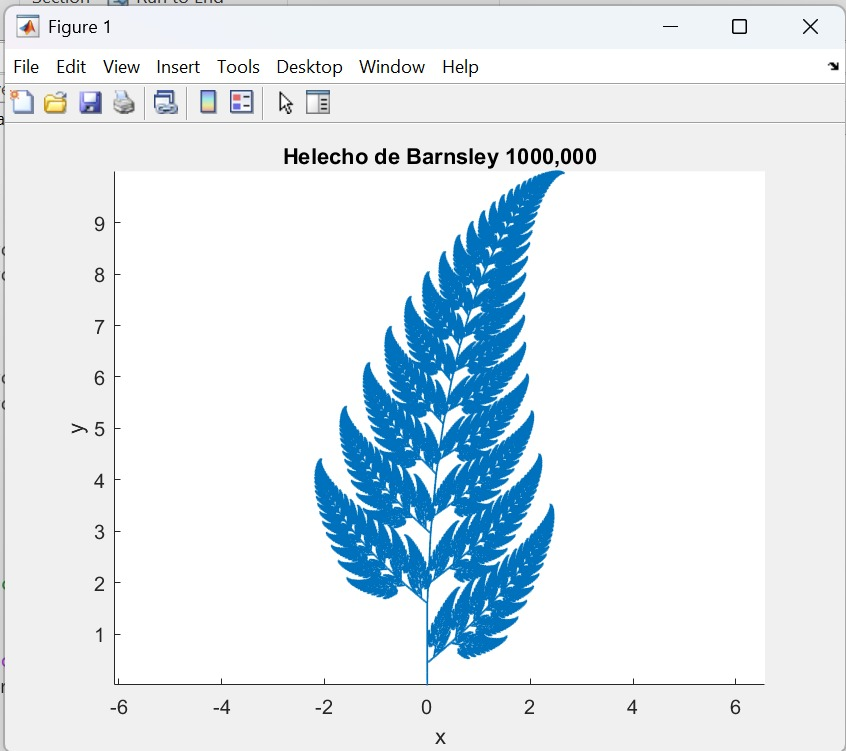
\includegraphics[width=0.75\textwidth]{helecho_1_000_000.jpeg}
    \caption{Helecho de Barnsley generado con 1\,000\,000 de puntos.}
    \label{fig:barnsley1000000}
\end{figure}


\subsection*{7.2 Fractal Estrella}

Para la generación de la Estrella se utilizaron dos transformaciones afines,
denominadas $T_1$ y $T_2$. Las probabilidades establecidas fueron:

\begin{equation}
P_1=0.912675
\end{equation}

\begin{equation}
P_2=0.087325.
\end{equation}

La primera transformacion es seleccionada con una frecuencia mucho mayor que
la segunda. El proceso iterativo modifica progresivamente la distribucion de
los puntos hasta formar la estructura correspondiente al fractal.

\subsubsection*{7.2.1 Resultados}

\begin{figure}[H]
    \centering
    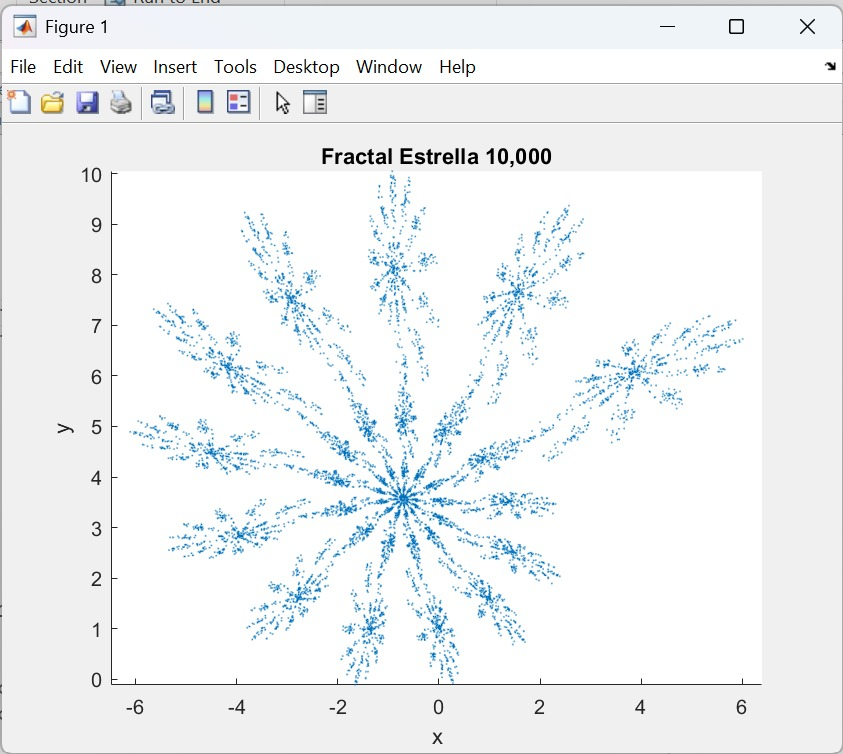
\includegraphics[width=0.75\textwidth]{estrella_10_000.jpeg}
    \caption{Estrella generada con 10\,000 puntos.}
    \label{fig:estrella10000}
\end{figure}

\begin{figure}[H]
    \centering
    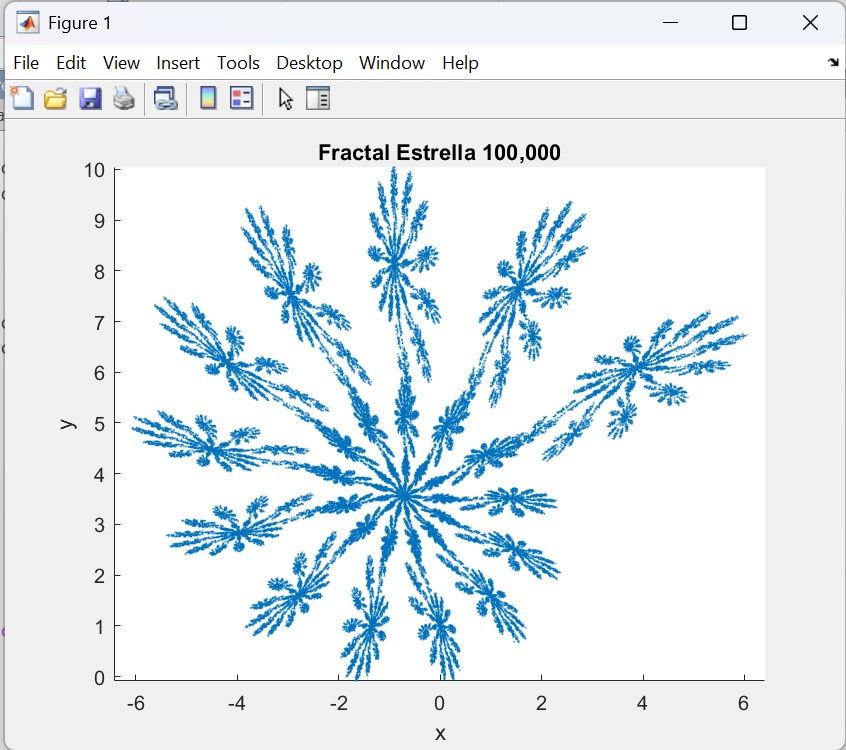
\includegraphics[width=0.75\textwidth]{estrella_100_000.jpeg}
    \caption{Estrella generada con 100\,000 puntos.}
    \label{fig:estrella100000}
\end{figure}

\begin{figure}[H]
    \centering
    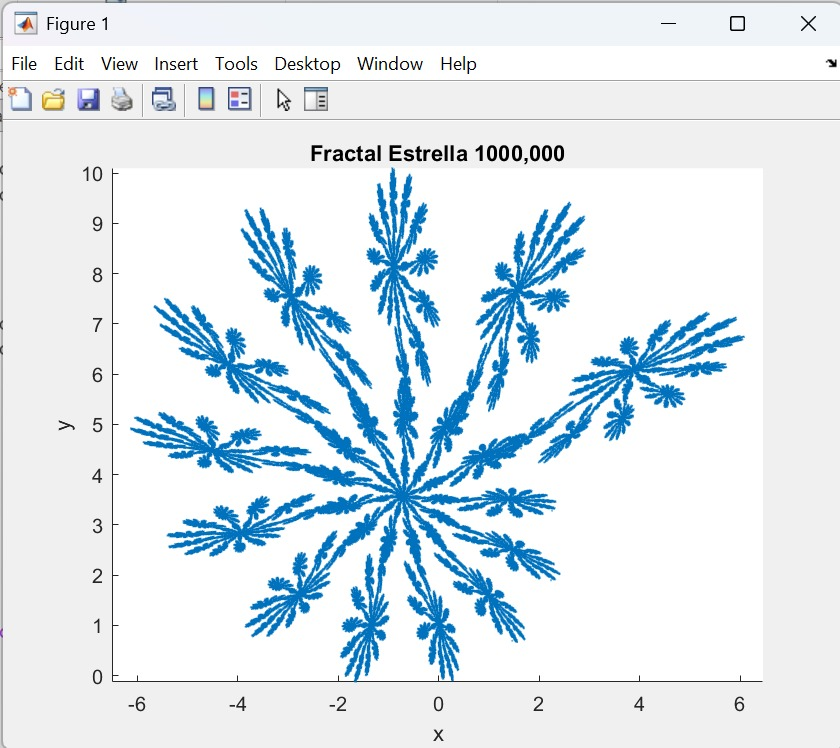
\includegraphics[width=0.75\textwidth]{estrella_1_000_000.jpeg}
    \caption{Estrella generada con 1\,000\,000 de puntos.}
    \label{fig:estrella1000000}
\end{figure}

\subsection*{7.3 Fractal Dragon}

Para el fractal Dragon se utilizaron dos transformaciones afines. Las probabilidades correspondientes fueron:

\begin{equation}
P_1=0.787473
\end{equation}

\begin{equation}
P_2=0.212527.
\end{equation}

En este caso, ambas transformaciones participan de manera significativa en
el proceso aunque la primera presenta una probabilidad de seleccion mayor.

\subsubsection*{7.3.1 Resultados}

\begin{figure}[H]
    \centering
    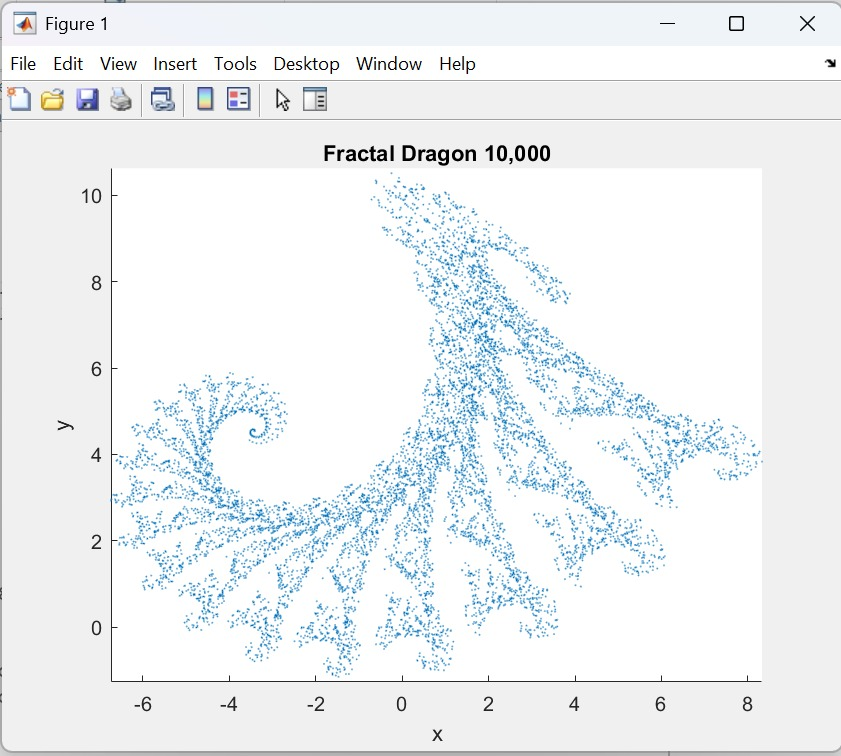
\includegraphics[width=0.75\textwidth]{dragon_10_000.jpeg}
    \caption{Dragon generado con 10\,000 puntos.}
    \label{fig:dragon10000}
\end{figure}

\begin{figure}[H]
    \centering
    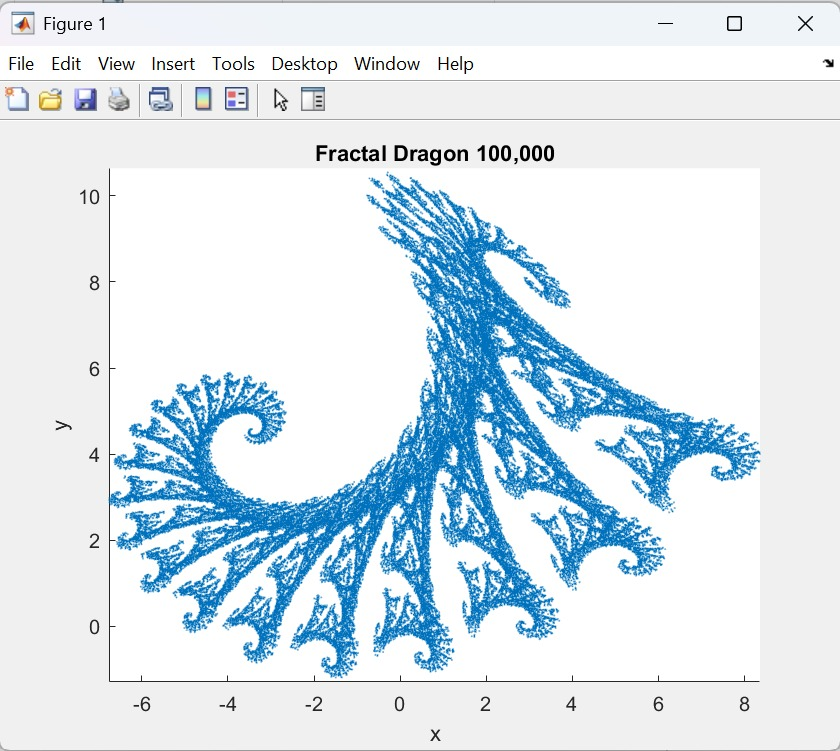
\includegraphics[width=0.75\textwidth]{dragon_100_000.jpeg}
    \caption{Dragon generado con 100\,000 puntos.}
    \label{fig:dragon100000}
\end{figure}

\begin{figure}[H]
    \centering
    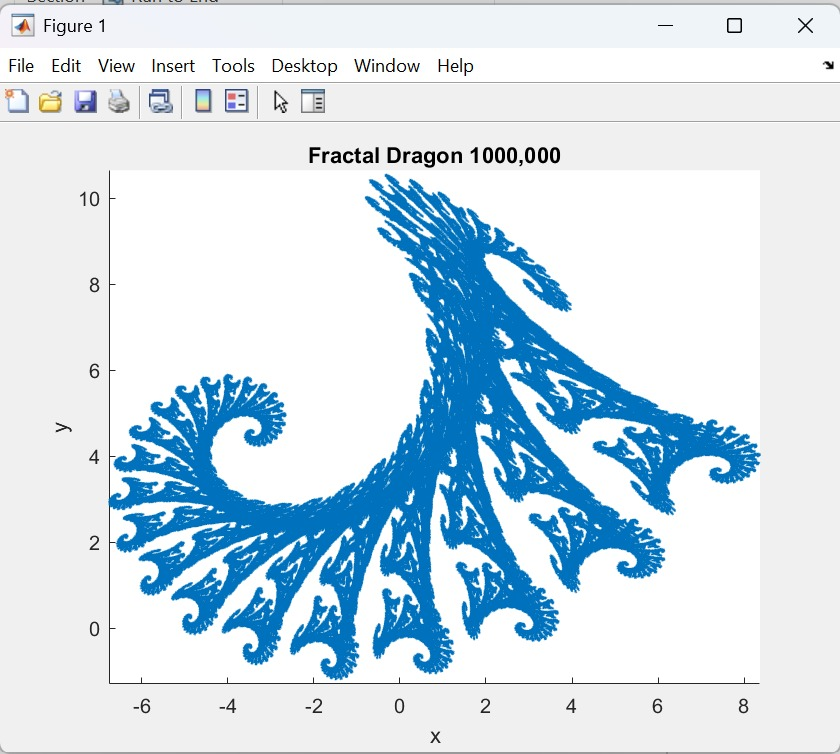
\includegraphics[width=0.75\textwidth]{dragon_1_000_000.jpeg}
    \caption{Dragon generado con 1\,000\,000 de puntos.}
    \label{fig:dragon1000000}
\end{figure}


\subsection*{7.4 Fractal Hoja de maple}

La Hoja de maple se construyo utilizando cuatro transformaciones afines. Las probabilidades proporcionadas fueron:

\begin{align}
P_1 &= 0.10,\\
P_2 &= 0.35,\\
P_3 &= 0.35,\\
P_4 &= 0.20.
\end{align}

Las transformaciones $T_2$ y $T_3$ presentan la mayor probabilidad de
seleccion, por lo que aparecen con mayor frecuencia durante la construcción
del fractal.

\subsubsection*{7.4.1 Resultados}

\begin{figure}[H]
    \centering
    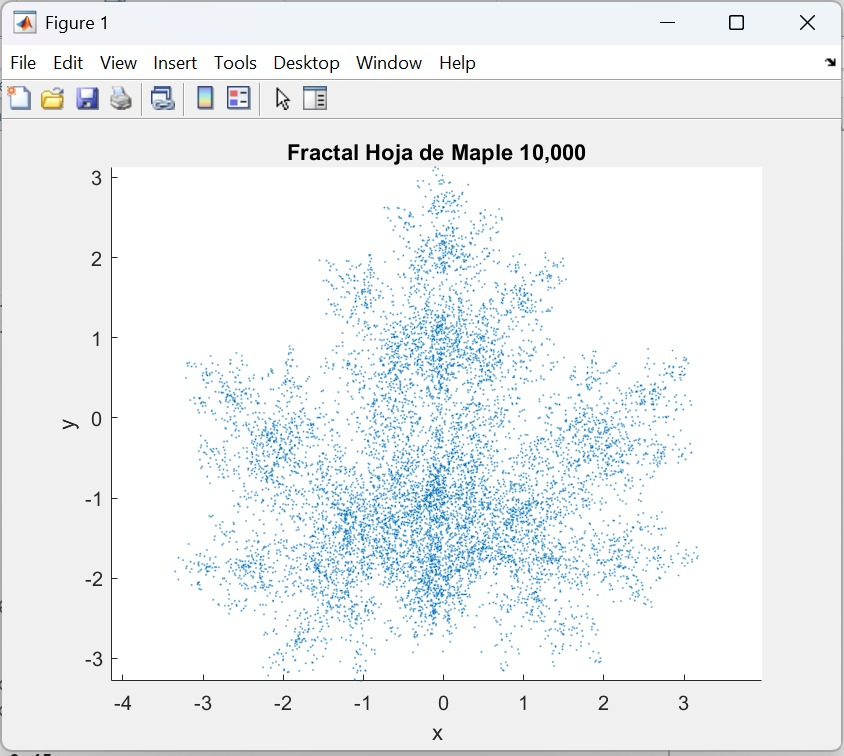
\includegraphics[width=0.75\textwidth]{maple_10_000.jpeg}
    \caption{Hoja de maple generada con 10\,000 puntos.}
    \label{fig:maple10000}
\end{figure}

\begin{figure}[H]
    \centering
    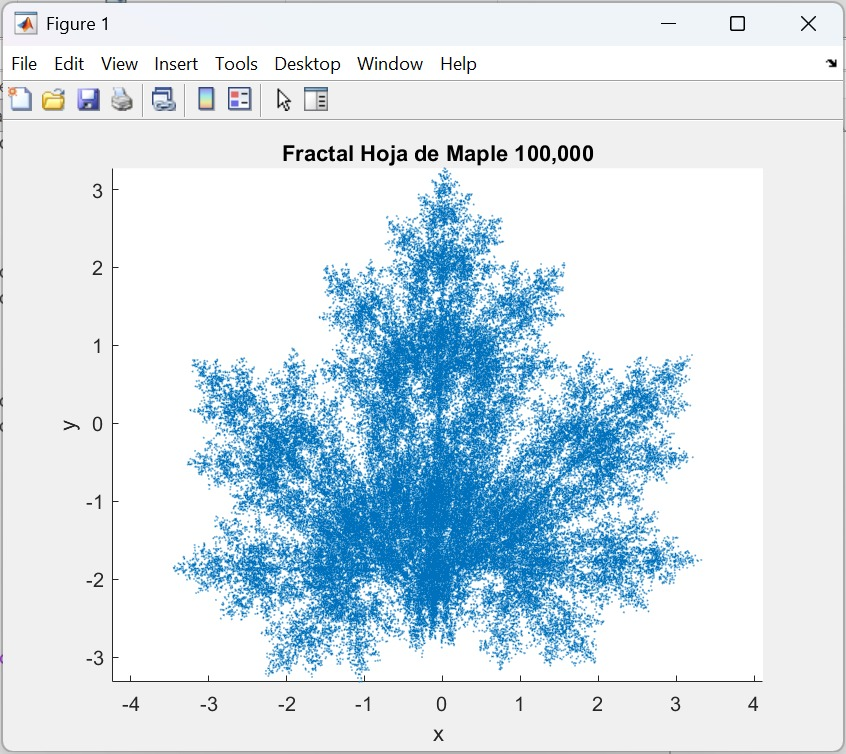
\includegraphics[width=0.75\textwidth]{maple_100_000.jpeg}
    \caption{Hoja de maple generada con 100\,000 puntos.}
    \label{fig:maple100000}
\end{figure}

\begin{figure}[H]
    \centering
    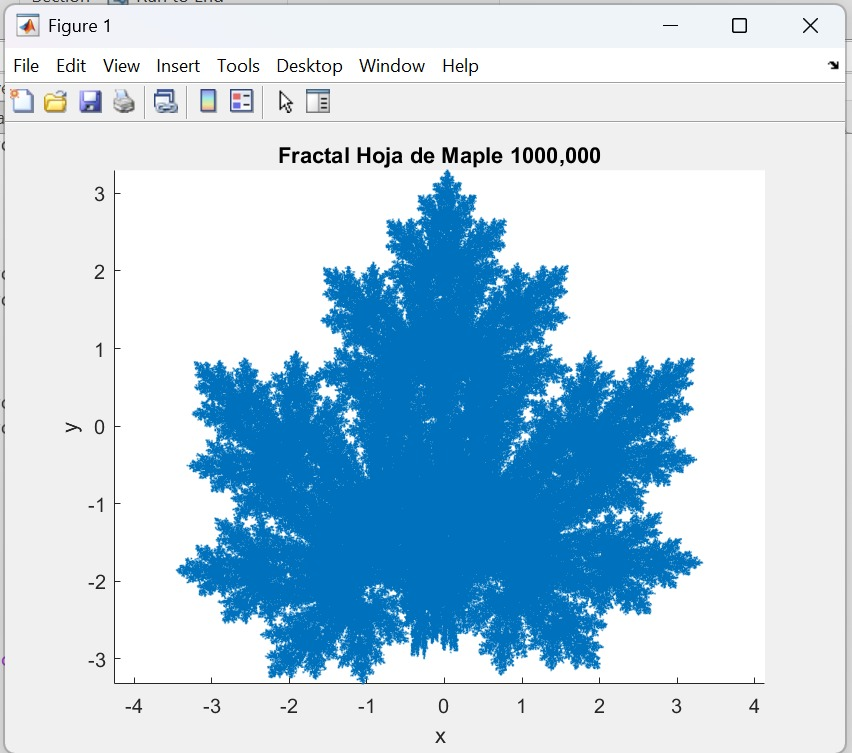
\includegraphics[width=0.75\textwidth]{maple_1_000_000.jpeg}
    \caption{Hoja de maple generada con 1\,000\,000 de puntos.}
    \label{fig:maple1000000}
\end{figure}


\subsection*{7.5 Triangulo de Sierpinski}

Para el Triangulo de Sierpinski se utilizaron tres funciones:

\begin{align}
f_1(x,y)&=(0.5x+1,\;0.5y+1),\\
f_2(x,y)&=(0.5x+1,\;0.5y+50),\\
f_3(x,y)&=(0.5x+50,\;0.5y+50).
\end{align}

Las tres transformaciones tienen la misma probabilidad:

\begin{equation}
P_1=P_2=P_3=\frac{1}{3}.
\end{equation}

Debido a esta distribucion uniforme, cada una de las transformaciones tiene
la misma posibilidad de ser seleccionada.

\subsection*{7.5.1 Resultados}

\begin{figure}[H]
    \centering
    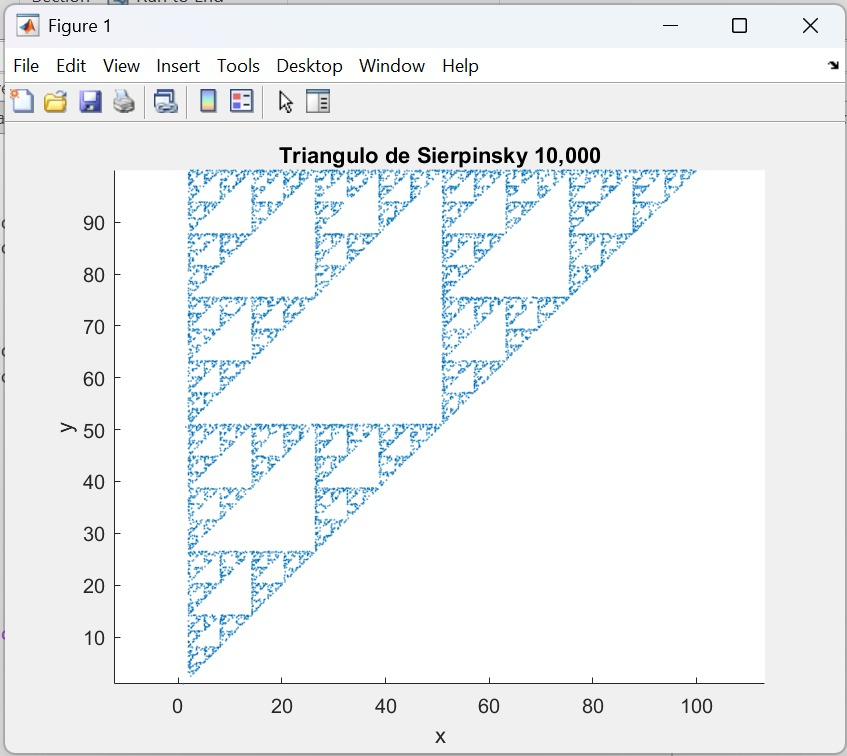
\includegraphics[width=0.75\textwidth]{triangulo_10_000.jpeg}
    \caption{Triangulo de Sierpinski generado con 10\,000 puntos.}
    \label{fig:sierpinski10000}
\end{figure}

\begin{figure}[H]
    \centering
    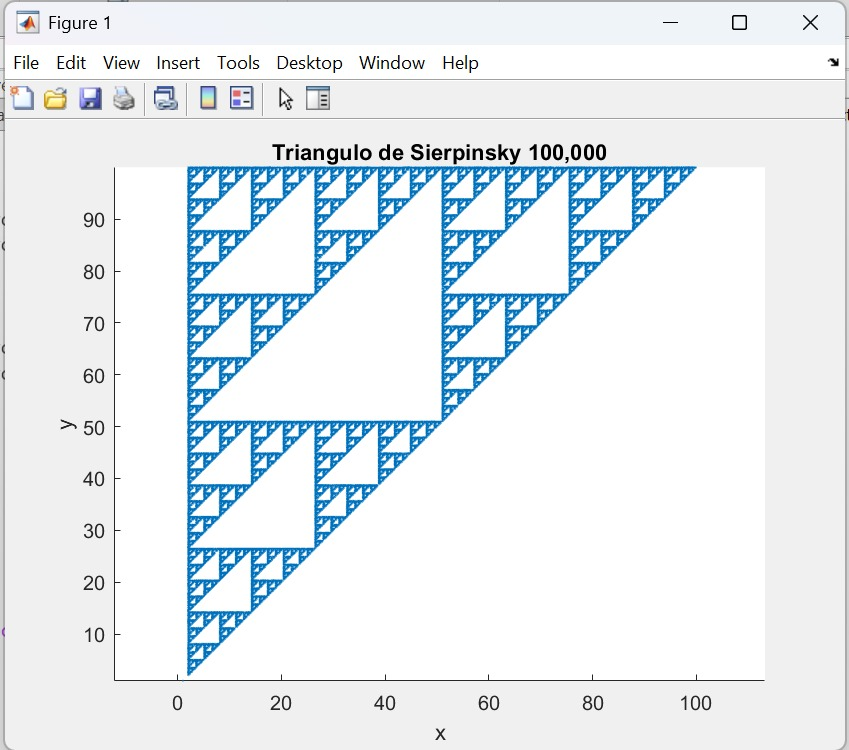
\includegraphics[width=0.75\textwidth]{triangulo_100_000.jpeg}
    \caption{Triangulo de Sierpinski generado con 100\,000 puntos.}
    \label{fig:sierpinski100000}
\end{figure}

\begin{figure}[H]
    \centering
    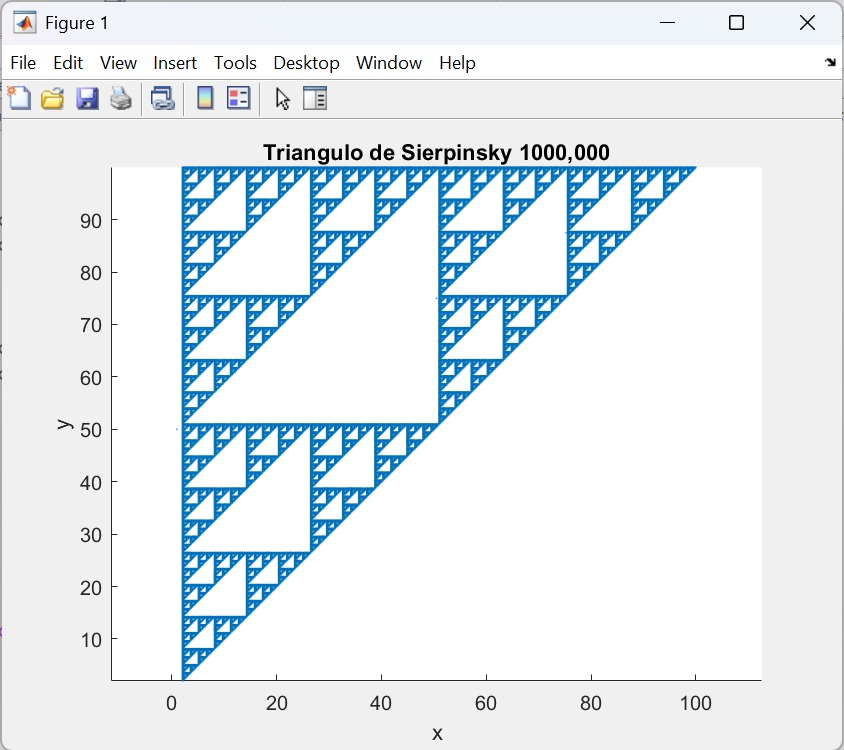
\includegraphics[width=0.75\textwidth]{triangulo_1_000_000.jpeg}
    \caption{Triangulo de Sierpinski generado con 1\,000\,000 de puntos.}
    \label{fig:sierpinski1000000}
\end{figure}


\subsection*{7.6 Variante de Sierpinski}

Se genero tambien una variante del fractal de Sierpinski utilizando tres
transformaciones.

\begin{equation}
T_1=
\begin{pmatrix}
0.5 & 0\\
0 & 0.5
\end{pmatrix},
\end{equation}

\begin{equation}
T_2=
\begin{pmatrix}
0 & -0.5\\
0.5 & 0
\end{pmatrix},
\end{equation}

\begin{equation}
T_3=
\begin{pmatrix}
0 & -0.5\\
0.5 & 0
\end{pmatrix}.
\end{equation}

Al utilizar probabilidades uniformes, las tres transformaciones tienen la
misma posibilidad de aparecer en cada iteracion.

\subsubsection*{7.6.1 Resultados}

\begin{figure}[H]
    \centering
    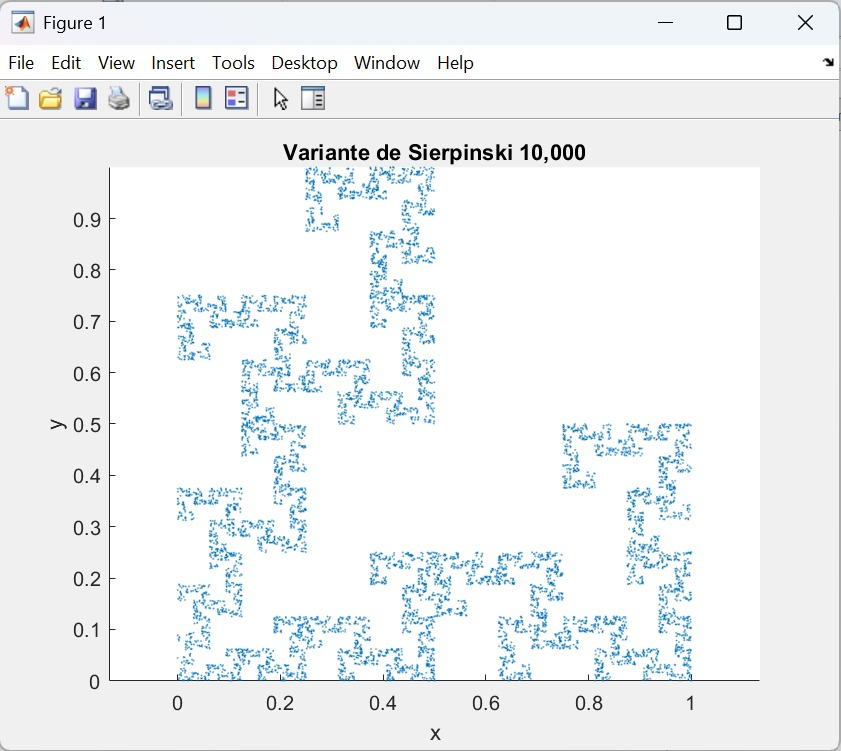
\includegraphics[width=0.75\textwidth]{variante_10_000.jpeg}
    \caption{Variante del Triangulo de Sierpinski generado con 10\,000 puntos.}
    \label{fig:variante10000}
\end{figure}

\begin{figure}[H]
    \centering
    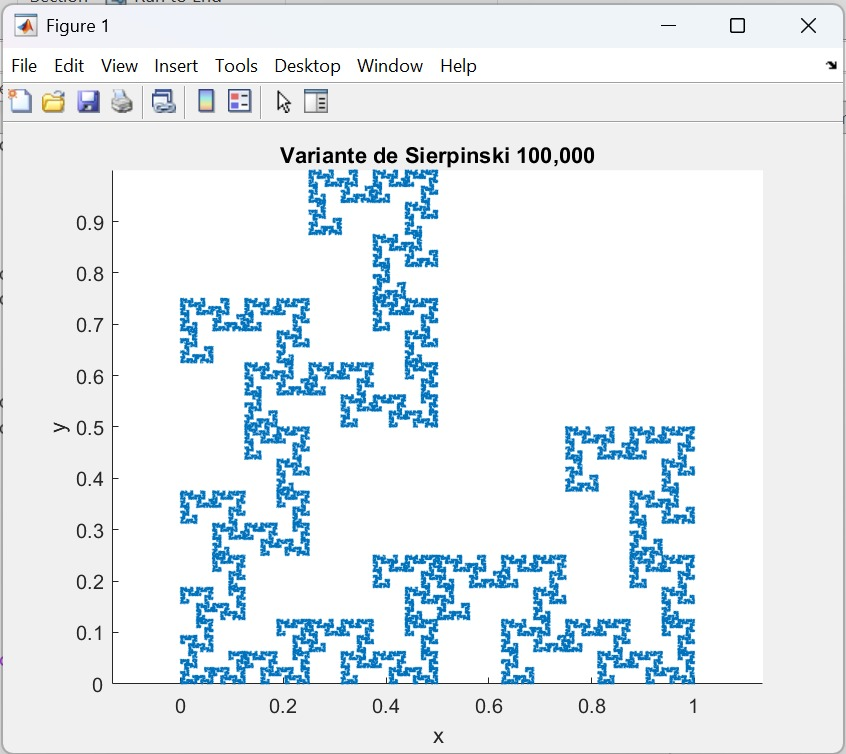
\includegraphics[width=0.75\textwidth]{variante_100_000.jpeg}
    \caption{Variante del Triangulo de Sierpinski generado con 100\,000 puntos.}
    \label{fig:variante100000}
\end{figure}

\begin{figure}[H]
    \centering
    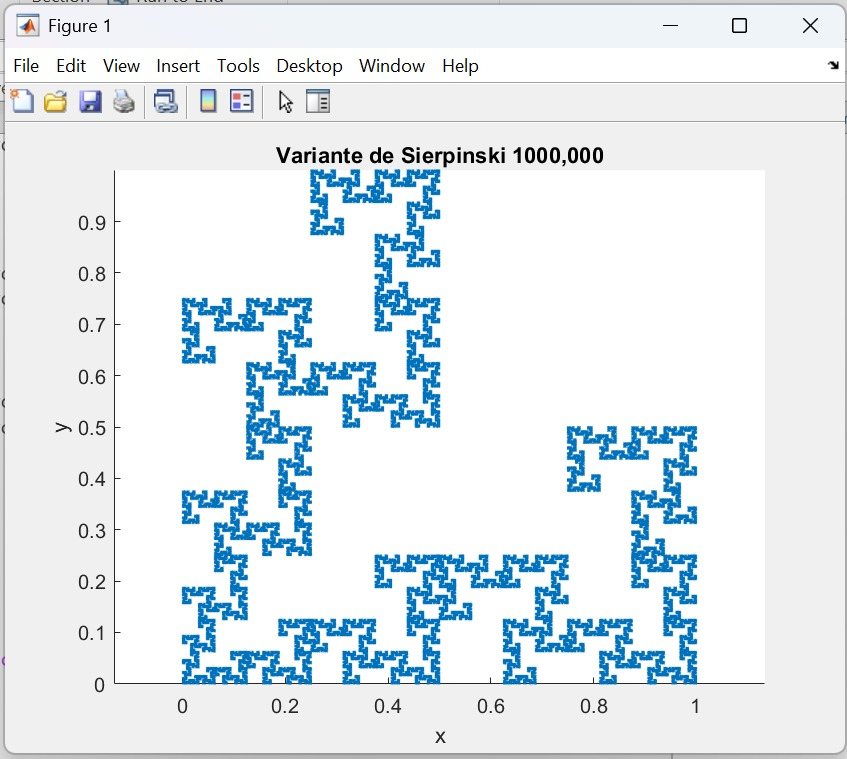
\includegraphics[width=0.75\textwidth]{variante_1_000_000.jpeg}
    \caption{Variante del Triangulo de Sierpinski generado con 1\,000\,000 de puntos.}
    \label{fig:variante1000000}
\end{figure}


\subsection*{7.7 Fractal Cristal}

Para generar el fractal Cristal se utilizaron tres transformaciones afines. El proceso iterativo permitio observar cómo la repeticion de estas operaciones genera una estructura geometrica con patrones repetitivos.

\subsubsection*{7.7.1 Resultados}

\begin{figure}[H]
    \centering
    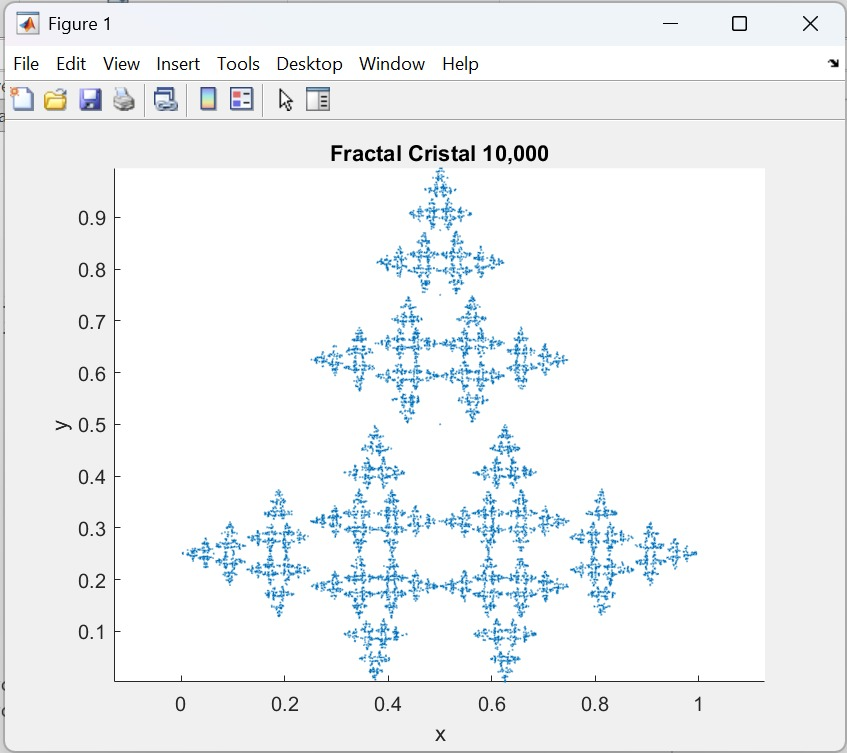
\includegraphics[width=0.75\textwidth]{cristal_10_000.jpeg}
    \caption{Fractal Cristal generado con 10\,000 puntos.}
    \label{fig:cristal10000}
\end{figure}

\begin{figure}[H]
    \centering
    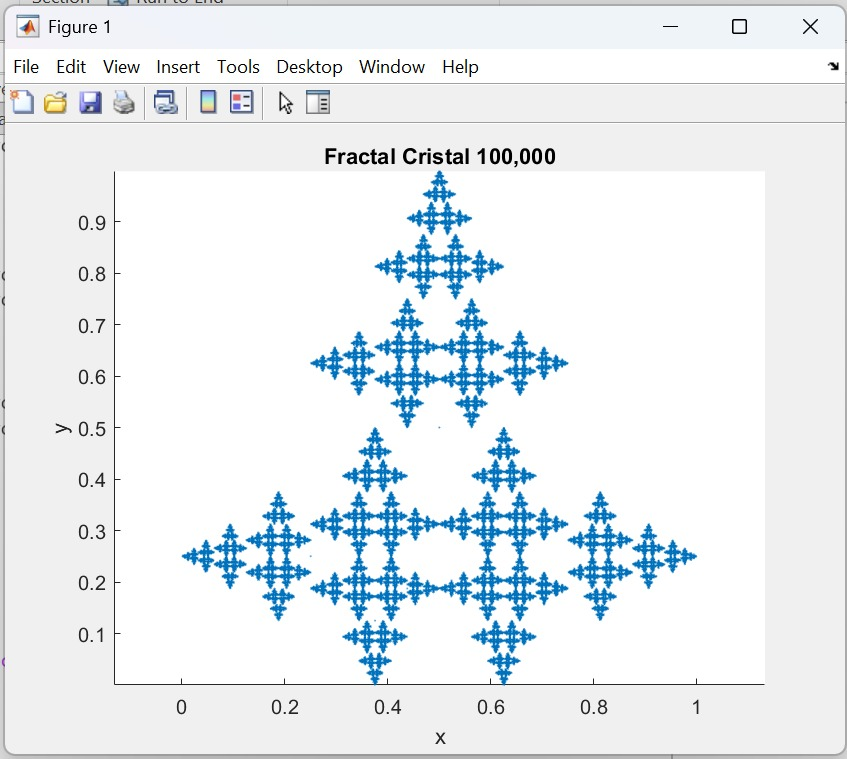
\includegraphics[width=0.75\textwidth]{cristal_100_000.jpeg}
    \caption{Fractal Cristal generado con 100\,000 puntos.}
    \label{fig:cristal100000}
\end{figure}

\begin{figure}[H]
    \centering
    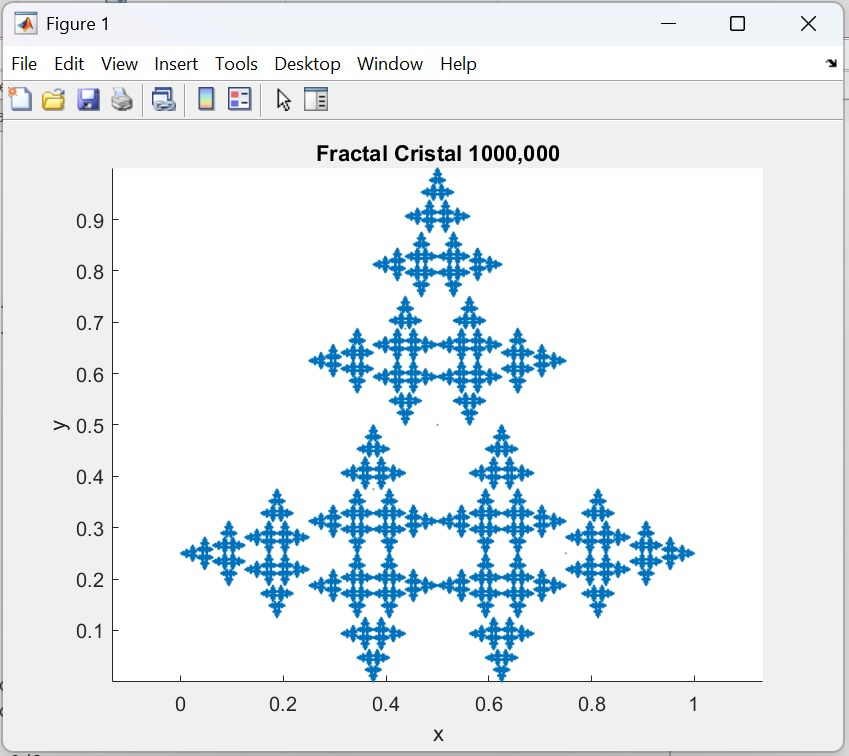
\includegraphics[width=0.75\textwidth]{cristal_1_000_000.jpeg}
    \caption{Fractal Cristal generado con 1\,000\,000 de puntos.}
    \label{fig:cristal1000000}
\end{figure}


\subsection*{7.8 Fractal copo de nieve}

Para generar el fractal copo de nieve se utilizaron seis transformaciones
afines, cada una definida mediante sus respectivos coeficientes de
transformacion y desplazamiento. Estas transformaciones permiten reducir
la escala de los puntos y ubicarlos en diferentes regiones del plano.

\subsubsection*{7.8.1 Resultados}

\begin{figure}[H]
    \centering
    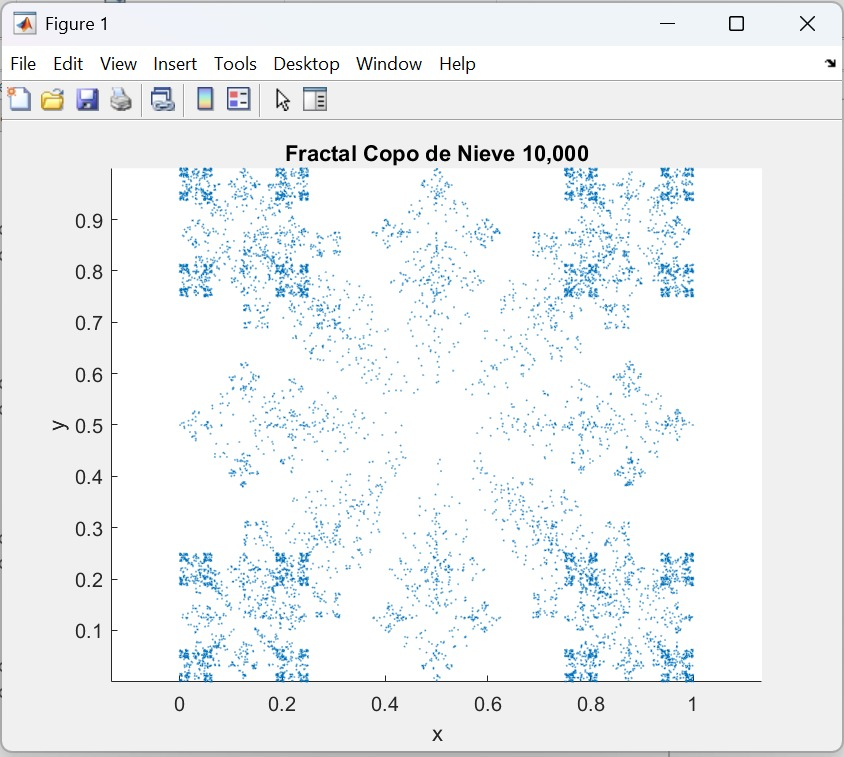
\includegraphics[width=0.75\textwidth]{copo_10_000.jpeg}
    \caption{Fractal copo de nieve generado con 10\,000 puntos.}
    \label{fig:copo10000}
\end{figure}

\begin{figure}[H]
    \centering
    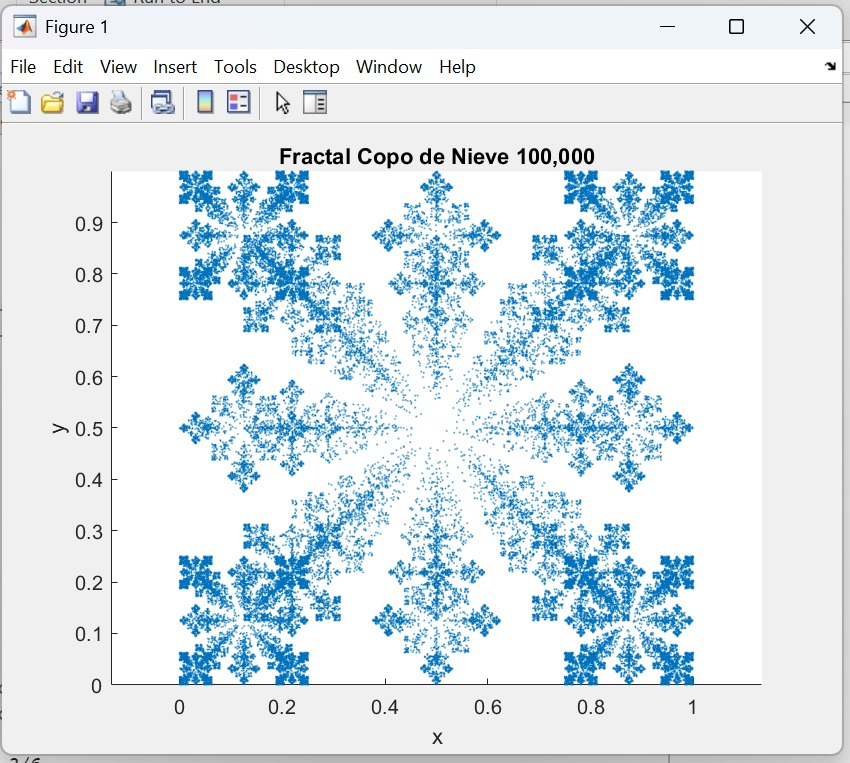
\includegraphics[width=0.75\textwidth]{copo_100_000.jpeg}
    \caption{Fractal copo de nieve generado con 100\,000 puntos.}
    \label{fig:copo100000}
\end{figure}

\begin{figure}[H]
    \centering
    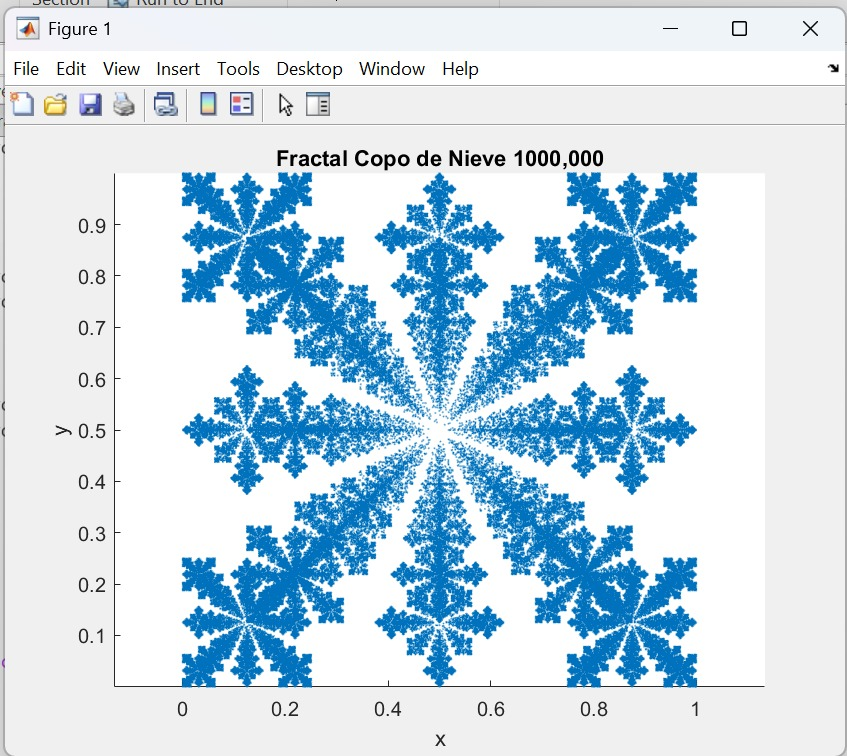
\includegraphics[width=0.75\textwidth]{copo_1_000_000.jpeg}
    \caption{Fractal copo de nieve generado con 1\,000\,000 de puntos.}
    \label{fig:copo1000000}
\end{figure}


\subsection*{7.9 Fractal Rama}

El fractal Rama fue generado mediante tres transformaciones que comparten
un factor de escala de $0.382$ y presentan diferentes desplazamientos. La caracteristica principal de este fractal es que la estructura global
aparece como consecuencia de la repeticion de patrones locales.

\subsubsection*{7.9.1 Resultados}

\begin{figure}[H]
    \centering
    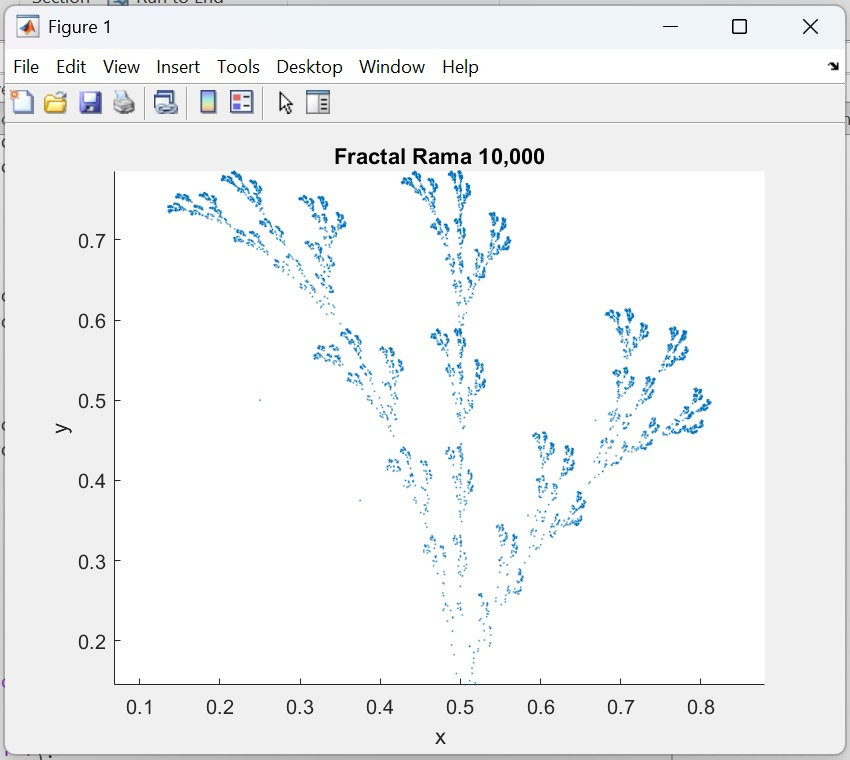
\includegraphics[width=0.75\textwidth]{rama_10_000.jpeg}
    \caption{Fractal Rama generado con 10\,000 puntos.}
    \label{fig:rama10000}
\end{figure}

\begin{figure}[H]
    \centering
    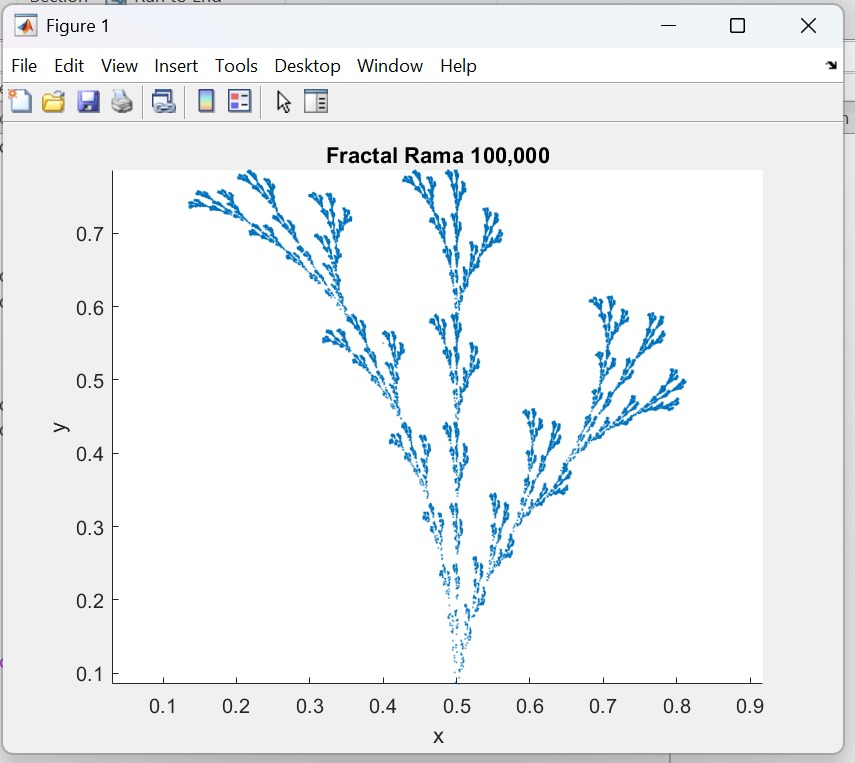
\includegraphics[width=0.75\textwidth]{rama_100_000.jpeg}
    \caption{Fractal Rama generado con 100\,000 puntos.}
    \label{fig:rama100000}
\end{figure}

\begin{figure}[H]
    \centering
    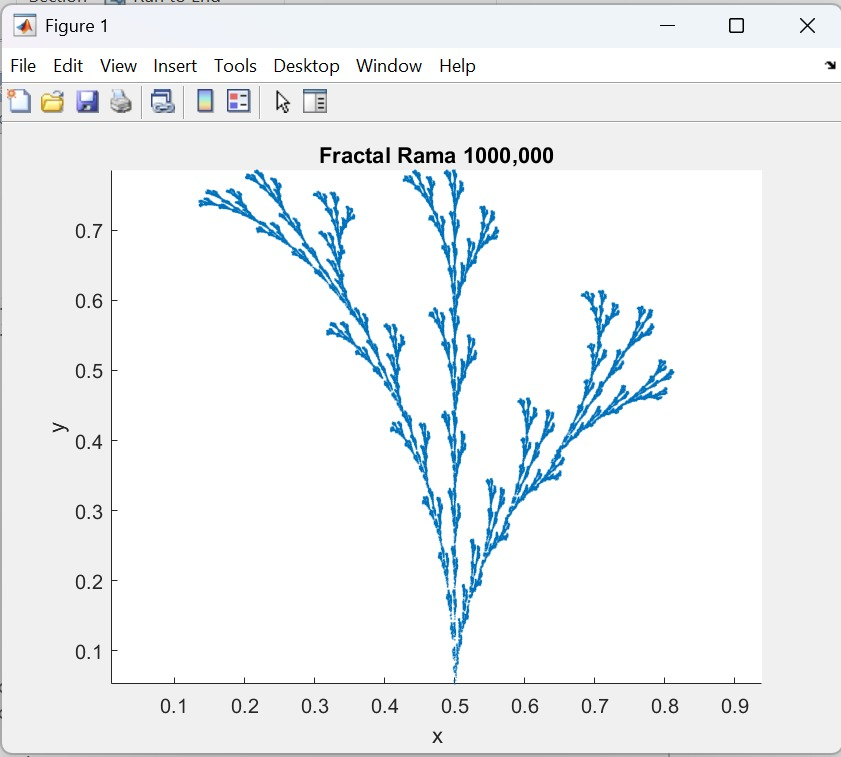
\includegraphics[width=0.75\textwidth]{rama_1_000_000.jpeg}
    \caption{Fractal Rama generado con 1\,000\,000 de puntos.}
    \label{fig:rama1000000}
\end{figure}


\subsection*{7.10 Pentagono de Sierpinski}

Para el Pentagono de Sierpinski se utilizaron cinco transformaciones. Las transformaciones tienen un factor de contraccion comun de $0.382$ y
diferentes desplazamientos, relacionados con las posiciones que ocupan las
distintas regiones del pentagono.

\subsubsection*{7.10.1 Resultados}

\begin{figure}[H]
    \centering
    \includegraphics[width=0.75\textwidth]{pentagono_10_000.jpeg}
    \caption{Fractal Pentagono de Sierpinski generado con 10\,000 puntos.}
    \label{fig:pentagono10000}
\end{figure}

\begin{figure}[H]
    \centering
    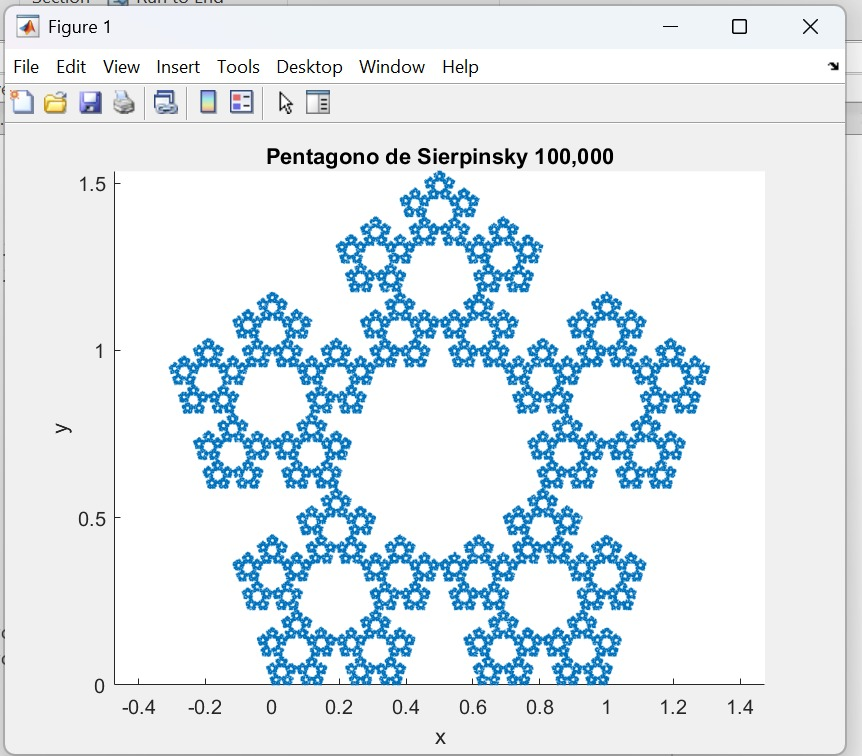
\includegraphics[width=0.75\textwidth]{pentagono_100_000.jpeg}
    \caption{Fractal Pentagono de Sierpinski generado con 100\,000 puntos.}
    \label{fig:pentagono100000}
\end{figure}

\begin{figure}[H]
    \centering
    \includegraphics[width=0.75\textwidth]{pentagono_1_000_000.jpeg}
    \caption{Fractal Pentagono de Sierpinski generado con 1\,000\,000 de puntos.}
    \label{fig:pentagono1000000}
\end{figure}


\section*{8. Análisis del tiempo de procesamiento}

Los tiempos obtenidos experimentalmente deberan registrarse en la siguiente
tabla.

\begin{table}[H]
\centering
\caption{Tiempo de procesamiento de los fractales en $[s]$.}
\label{tab:tiempos}
\begin{tabular}{lccc}
\toprule
\textbf{Fractal} &
\textbf{10\,000} &
\textbf{100\,000} &
\textbf{1\,000\,000} \\
\midrule
Helecho de Barnsley & 0.00367 & 0.00495 & 0.03075 \\
Estrella            & 0.00152 & 0.00394 & 0.02771 \\
Dragón              & 0.00163 & 0.00414 & 0.02939 \\
Hoja de maple       & 0.00259 & 0.00581 & 0.03990 \\
Sierpinski          & 0.00186 & 0.00507 & 0.03569 \\
Sierpinski variante & 0.00186 & 0.00511 & 0.03740 \\
Cristal             & 0.00369 & 0.01021 & 0.05802 \\
Copo de nieve       & 0.00619 & 0.01006 & 0.06696 \\
Rama                & 0.00697 & 0.00792 & 0.05963 \\
Pentágono           & 0.00513 & 0.00950 & 0.06557 \\
\bottomrule
\end{tabular}
\end{table}

Es importante destacar que estos valores pueden variar dependiendo de la computadora utilizada y las condiciones en que se ejecutaron las simulaciones. Sin embargo, se observo que el tiempo de procesamiento aumenta con el numero de puntos utilizados y que los fractales con mayor cantidad de transformaciones tienden a requerir más tiempo para su generación.


\section*{9. Conclusiones}

La utilizacion de MATLAB ha sido fundamental en la realizacion de este trabajo ya que nos es útil para la generación y visualizacion de variables aleatorias con distribucion uniforme, la iteración de procesos asi como la visualizacion de graficas e imagenes Los resultados obtenidos permiten comprobar que estructuras geometricas complejas pueden generarse a partir de un conjunto reducido de reglas matematicas.


\section*{10. Bibliografia}

\begin{thebibliography}{9}

\bibitem{practica}
Facultad de Ingeniería, Universidad Nacional Autónoma de México,
\textit{Proyecto 1: Fractales, Temas Selectos de Matemáticas:
Probabilidad}, Semestre 2027-1. \\
\bibitem{Optimizacion en fractales}
PhD thesis, Universidad Politécnica de Madrid, 2022. \\
\textit{Garcia-Miguel Fernandez}
\end{thebibliography}
\end{document}